\documentclass[a4paper,12pt]{article}
\usepackage[english,ukrainian,russian]{babel}
\linespread{1}
\usepackage{ucs}
\usepackage[utf8]{inputenc}
\usepackage[T2A]{fontenc}
\usepackage[paper=portrait,pagesize]{typearea}
\usepackage{amsmath}
\usepackage{bigints}
\usepackage{amsfonts}
\usepackage{graphicx}
\usepackage{amssymb}
\usepackage{cancel}
\usepackage{gensymb}
\usepackage{multirow}
\usepackage{rotate} 
\usepackage{pdflscape}
\usepackage{bigstrut}
\usepackage[pageanchor]{hyperref}
\usepackage{chngpage}
\newcommand{\dx}{\textbf{d}x}
\newcommand{\dt}{\textbf{d}t}
\newcommand{\du}{\textbf{d}u}
\newcommand{\dv}{\textbf{d}v}
\newcommand{\dy}{\textbf{d}y}
\newcommand{\ds}{\textbf{d}s}
\newcommand{\dz}{\textbf{d}z}
\newcommand{\arch}{\textrm{arcch}}
\newcommand{\arsh}{\textrm{arcsh}}
\newcommand{\dint}{\displaystyle\int}
\newcommand\tab[1][1cm]{\hspace*{#1}}
\newcommand{\RomanNumeralCaps}[1]{\MakeUppercase{\romannumeral #1}}
\newcommand{\dsum}{\displaystyle\sum}
\usepackage[left=20mm, top=20mm, right=15mm, bottom=15mm, nohead, nofoot]{geometry}
\usepackage{verbatim}
\usepackage{enumerate}
\usepackage{listings}
\usepackage{xcolor}

\definecolor{codegreen}{rgb}{0,0.6,0}
\definecolor{codegray}{rgb}{0.5,0.5,0.5}
\definecolor{codepurple}{rgb}{0.58,0,0.82}
\definecolor{backcolour}{rgb}{0.95,0.95,0.92}

\lstdefinestyle{mystyle}{
	backgroundcolor=\color{backcolour},   
	commentstyle=\color{codegreen},
	keywordstyle=\color{blue},
	numberstyle=\tiny\color{codegray},
	stringstyle=\color{red},
	basicstyle=\ttfamily\footnotesize,
	breakatwhitespace=false,         
	breaklines=true,                 
	captionpos=b,                    
	keepspaces=true,                 
	numbers=none,                    
	numbersep=5pt,                  
	showspaces=false,                
	showstringspaces=false,
	showtabs=false,                  
	tabsize=4,
	frame=shadowbox
}

\lstset{style=mystyle}

\begin{document}
	\begin{center}
		{\Large \bfseries \textsc{Лабораторна робота №8}}\\
		\hrulefill\\
		\Large \textsc{ФІ-12 Завалій Олександр\\ Варіант №5}
	\end{center}
	\begin{center}
		\section*{\bfseries{Завдання}}
	\end{center} 
	\textbf{Предметна область:} \\
	Навчально-методичне управління (облік площі приміщень). \\
	\textbf{Основні предметно-значущі сутності:} \\
	Приміщення, Підрозділи. \\
	\textbf{Основні предметно-значущі атрибути сутностей:}
	\begin{enumerate}
		\item[-] \textbf{Приміщення}: назва або номер приміщення, вид приміщення (аудиторія, кабінет і т.п.), площа, кількість посадочних місць, підрозділ. 
		\item[-] \textbf{Підрозділи}: назва, вид підрозділу.
	\end{enumerate}
	\textbf{Основні вимоги до функцій системи:}
	\begin{enumerate}
		\item[-] Вибрати назви або номери приміщень за підрозділами;
		\item[-] Підрахувати загальну площу навчальних аудиторій по приміщеннях і в цілому по навчальному закладу;
		\item[-] Підрахувати загальну кількість посадочних місць для співробітників по підрозділам.
	\end{enumerate}
	\textbf{Тригери:}
	\begin{enumerate}
		\item На видалення запису з таблиці «Приміщення». Якщо для приміщення зазначено підрозділ, заборонити видалення запису.
		\item Створити представлення «Аудиторії» з полями «код приміщення», «назва приміщення», «підрозділ», в яку повинні входити приміщення виду «Аудиторія». Оновлювати представлення «Аудиторії».
	\end{enumerate}
	\textbf{Процедура:}\\
	Процедура повинна повертати кількість приміщень для зазначеного підрозділу. \\
	\begin{center}
		\textbf{Завдання для лабораторної роботи}
	\end{center}
    Створити тригери, які вказані у вашому завданні.

\newpage
	\begin{center}
		\section*{\bfseries{Реалізація завдання}}
	\end{center}
    \begin{center}
        \Large{Task \RomanNumeralCaps{1}}
    \end{center}
    \textbf{Створити тригер на видалення запису з таблиці «Приміщення». Якщо для приміщення зазначено підрозділ, заборонити видалення запису.}
	\begin{lstlisting}[language=SQL]
	CREATE TRIGGER DeleteLine ON Room INSTEAD OF DELETE
	AS BEGIN
		DECLARE @SubdId INT;
		DECLARE @count INT;
		SELECT @SubdId = SubdivisionId FROM DELETED;
		SELECT @count = COUNT(*) FROM Subdivision WHERE SubdivisionId = @SubdId;
		IF @count = 0
			DELETE FROM Room WHERE RoomId = @SubdId;
		ELSE
			THROW 51000, 'Can not delete - Room is referenced in other tables', 1;
	END

	DELETE FROM Room WHERE RoomId='1'
	GO
	\end{lstlisting}
	\begin{figure}[h!]
		\begin{minipage}[h]{1\linewidth}
			\centering
			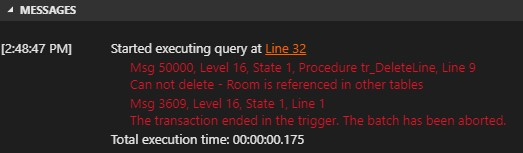
\includegraphics[width=0.6\linewidth]{Prt sc/Figure_1.jpg}  
		\end{minipage}
		\caption{Спроба видалити запис під номером "1".}
	\end{figure}
	
	\begin{center}
        \Large{Task \RomanNumeralCaps{2}}
    \end{center}
	\textbf{Створити представлення «Аудиторiї» з полями «код примiщення», «назва примiщен-
	ня», «пiдроздiл», в яку повиннi входити примiщення виду «Аудиторiя». Оновлювати
	представлення «Аудиторiї».} \\
	Спочатку створемо представлення «Аудиторiї» з відповідними полями.
	\begin{lstlisting}[language=SQL]
	CREATE VIEW Audience AS
	SELECT RoomId, TypeOfRoom, Rm.SubdivisionId FROM Subdivision Sb, Room Rm
		where Sb.SubdivisionId=Rm.SubdivisionId and Rm.TypeOfRoom='Audience'
	GO
	
	SELECT *
	FROM Audience
	GO
	\end{lstlisting}
\newpage
	\begin{figure}[h!]
		\begin{minipage}[h]{1\linewidth}
			\centering
			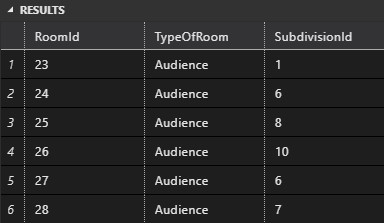
\includegraphics[width=0.6\linewidth]{Prt sc/Figure_2.jpg}  
		\end{minipage}
		\caption{Представлення «Аудиторiї».}
	\end{figure}
\end{document}